% Retrospective supporting checks; no new primary confidence claim.
\subsection{Retrospective influence and coordinate-recovery diagnostics}\label{app:review-diagnostics}
These descriptive checks were added after the original study. They reuse the declared
paired repetitions and do not change the primary estimates, margins, or comparison
families. For each of the 41 primary contrasts, we compute bias-corrected sample
skewness and delete each repetition once. Each deletion recomputes the Student
interval with 23 remaining repetitions, 22 degrees of freedom, and the original
family size (29 or 12). The range of deletion endpoints is an influence diagnostic,
not a confidence interval or an additional simultaneous-coverage claim.
Table~\ref{tab:review-paired} shows the four Van der Pol comparisons; the complete
descriptive results accompany the executable artifact.
All four Van der Pol comparisons retain lower endpoints above the fixed practical
margin after any one-repetition deletion. This does not establish a distribution-free
mean guarantee or remove the normal-approximation qualification of the primary analysis.
\begin{table}[htbp]
\caption{Retrospective Van der Pol influence diagnostics. Lower endpoints are multiplied
by $10^3$; the fixed margin on this scale is $0.148907$. Skewness is the bias-corrected
Fisher--Pearson sample coefficient. The minimum deletion lower endpoint is the smallest
over all 24 one-repetition deletions. The final column counts individual paired
differences exceeding the margin; it is not a mean-effect confidence statement.}
\label{tab:review-paired}
\centering\small\setlength{\tabcolsep}{4pt}
% Retrospective diagnostics; generated by scripts/review_diagnostics.py.
\begin{tabular}{llrrrr}
\toprule
Control & $M$ & Skewness & Original lower & Min. deletion lower & $D_r>\delta$ \\
\midrule
Raw & 64 & -0.07 & 1.7369 & 1.7278 & 24/24 \\
Affine local & 64 & 2.69 & 0.2755 & 0.2685 & 24/24 \\
Raw & 256 & 0.01 & 0.7550 & 0.7524 & 24/24 \\
Affine local & 256 & 0.33 & 0.1810 & 0.1786 & 23/24 \\
\bottomrule
\end{tabular}

\end{table}
\begin{figure}[htbp]
\centering
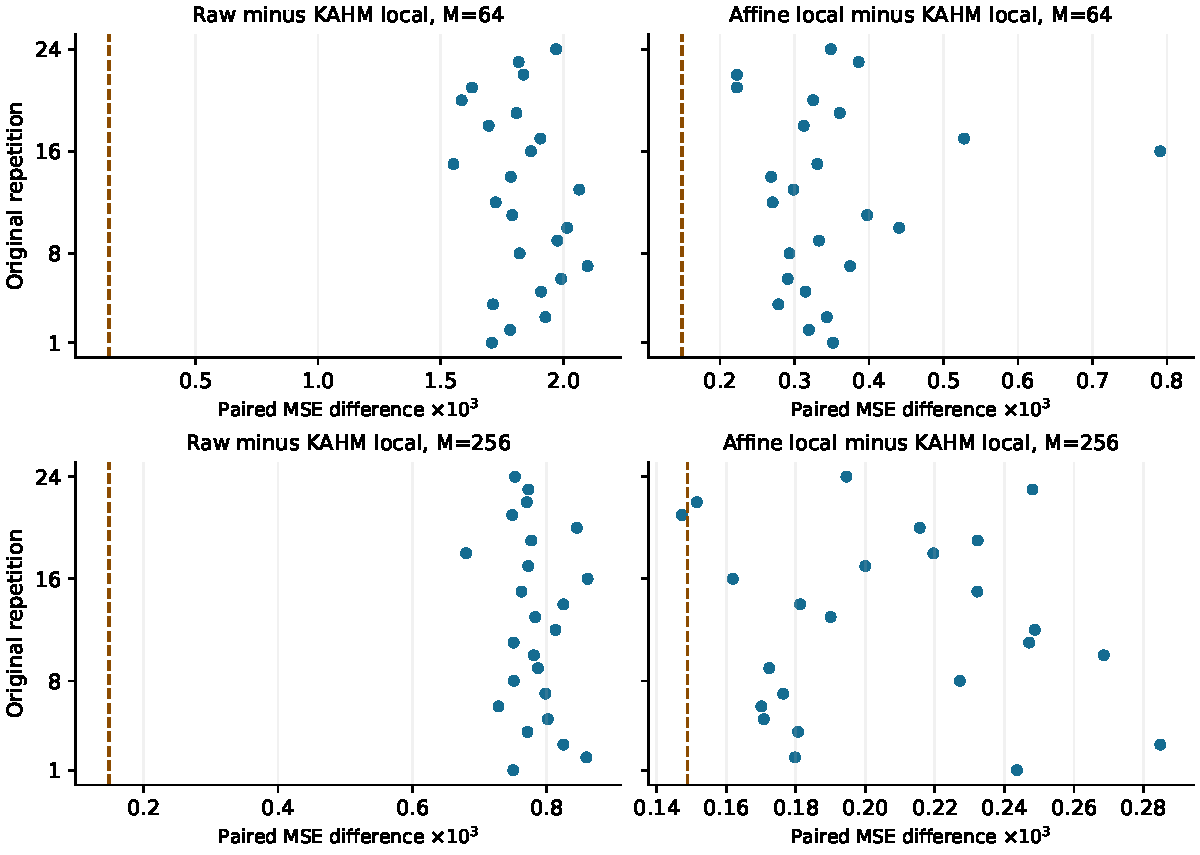
\includegraphics[width=.96\textwidth]{generated/figures/review_paired_differences.pdf}
\caption{The 24 original paired differences for each Van der Pol capacity comparison,
in units of $10^{-3}$ MSE. The dashed line is the frozen practical margin.
No resampling, refitting, or new primary analysis is performed.}
\label{fig:review-paired}
\end{figure}

We also inspect the 120 first-stage primary banks and 72 capacity banks from a
completed computational reproduction using the published seeds. No bank or head is
refitted for these diagnostics. Replayed test inputs, targets, and groups are checked
against their recorded hashes before the original feature map is evaluated.
Let $A$ vertically stack the $P_c^\top$ matrices. Proposition~\ref{prop:local-injectivity}
shows that positive gates and full column rank of $A$ suffice to recover the scaled
input from the gated local coordinates and gates:
division by $\phi_c$ recovers $P_c^\top(z-\mu_c)$, after which one solves for $z$.
A deficient stack does not establish information loss in the full code, because the
gates can carry additional information. Numerical ranks use the threshold
$\sigma_1\max\{\text{rows}(A),d\}\epsilon_{64}$; they are finite-precision diagnostics,
not exact rank proofs. Small singular values and small gates can make coordinate
recovery sensitive to perturbations. Test-sample gate minima are not population
lower bounds, and these computations do not guarantee a well-conditioned inverse
or easy decoding by any particular fitted head.
\begin{table}[htbp]
\caption{Retrospective diagnostics over 24 stored banks per row. Rank ranges concern
the stacked local bases in input dimension $d$. The smallest singular value and
gate entries are minima over the inspected banks (and, for gates, their original
test observations); $\kappa_2$ is the largest stack condition number. A dash means
that not every stack in that row has full numerical column rank. KAHM and affine
representations share the basis stack. Computational reproduction supplies no new
independent statistical replications.}
\label{tab:review-banks}
\centering\small\setlength{\tabcolsep}{3pt}
% Full column rank is sufficient; numerical ranks are diagnostics, not exact proofs.
\begin{tabular}{llrrrr}
\toprule
Phase / setting & Rank / $d$ & Min. $\sigma_d$ & Max. $\kappa_2$ & Min. $\phi^{\K}$ & Min. $\phi^{\A}$ \\
\midrule
First: Straight branch & 1/2 & $0$ & --- & $3.36\times10^{-25}$ & $2.56\times10^{-20}$ \\
First: Curved branch & 2/2 & $2.19\times10^{0}$ & $1.39\times10^{0}$ & $3.55\times10^{-28}$ & $8.97\times10^{-29}$ \\
First: Nonlinear AR & 12/12 & $6.20\times10^{-2}$ & $4.90\times10^{1}$ & $2.21\times10^{-35}$ & $2.36\times10^{-34}$ \\
First: Van der Pol & 12/12 & $1.60\times10^{-2}$ & $2.20\times10^{2}$ & $2.84\times10^{-45}$ & $9.43\times10^{-20}$ \\
First: Duffing & 12/12 & $1.33\times10^{-2}$ & $2.80\times10^{2}$ & $3.92\times10^{-43}$ & $3.11\times10^{-7}$ \\
Capacity: Nonlinear AR & 12/12 & $7.31\times10^{-2}$ & $4.19\times10^{1}$ & $9.97\times10^{-37}$ & $7.75\times10^{-37}$ \\
Capacity: Van der Pol & 12/12 & $1.60\times10^{-2}$ & $2.19\times10^{2}$ & $6.21\times10^{-44}$ & $1.56\times10^{-16}$ \\
Capacity: Duffing & 12/12 & $1.32\times10^{-2}$ & $2.84\times10^{2}$ & $5.38\times10^{-43}$ & $1.86\times10^{-8}$ \\
\bottomrule
\end{tabular}

\end{table}
